\documentclass[twocolumn,fleqn,8pt]{article}  % fleqn left alligns all equations. 
\usepackage[english]{babel} 
\usepackage[latin1]{inputenc} 
\usepackage{times} 			% Default times font style
\usepackage[T1]{fontenc} 	% Font encoding
\usepackage{amsmath} 		% Math package
\usepackage{mathtools} 		% Adds the declare paired 
							% delimeter command to make costom \abs and \norm
\usepackage{breqn}		 	% Adds dmath environment for automated brakeline
\usepackage{xfrac}			% Adds slanted fractions (sfrac)
\usepackage{cancel}			% Adds the cancel command, a slash through the symbol(s)
\usepackage{tabularx}		% Adds adjustable width on tabulars
\usepackage{cuted}			% Adds the \strip command, pagewidth text in a twocolumn
							% environment. 
\usepackage{hyperref}
							% Color library. The options allows using names of colors.
\usepackage[usenames,dvipsnames,svgnames]{xcolor}			
\usepackage{geometry}		% Change paper properties such as size. 
\usepackage{fancyhdr}		% Adds customizable headers and footers. 
\usepackage{tikz}
\usepackage{tikz-3dplot}		
\usepackage{blindtext}
\usepackage{titlesec}		% Can change properties of sections, such as color. 
\usepackage{colortbl}
\usepackage[justification=centering]{caption}

% Paper properties. 
\geometry{margin=2cm}
\setlength{\columnsep}{20pt}
\pagestyle{fancy}
\fancyhead[L]{Left }
\fancyhead[R]{Right }

% Assign some new column types. 
\newcolumntype{a}{>{\columncolor{LightCyan}}c}

% Change the definition of \vec to \mathbf
\renewcommand\vec[1]{\mathbf{#1}}
% Start costum \abs \norm 
\DeclarePairedDelimiter\abs{\lvert}{\rvert}%
\DeclarePairedDelimiter\norm{\lVert}{\rVert}%
% Swap the definition of \abs* and \norm*, so that \abs
% and \norm resizes the size of the brackets, and the 
% starred version does not.
\makeatletter
\let\oldabs\abs
\def\abs{\@ifstar{\oldabs}{\oldabs*}}
%
\let\oldnorm\norm
\def\norm{\@ifstar{\oldnorm}{\oldnorm*}}
\makeatother
% End costum \abs \norm 

% Change section formatting. 
\titleformat{\section}
{\color{MediumBlue}\normalfont\Large\bfseries}	% Properties of the title.
{\color{black}\thesection}{1em}{} 			% Properties of the number.
\titleformat{\subsection}
{\color{MediumBlue}\normalfont\large\bfseries}	% Properties of the title.
{\color{black}\thesubsection}{1em}{} 			% Properties of the number.
\titleformat{\subsubsection}
{\color{MediumBlue}\normalfont\large\bfseries}	% Properties of the title.
{\color{black}\thesubsubsection}{1em}{} 			% Properties of the number.

\begin{document}

% Skip the twocolumn environment. This is a hack. The extra "{}" are 
% needed to make the minipage options work. 
\twocolumn[{
	
	\begin{@twocolumnfalse}
	
	\noindent\LARGE{\color{MediumBlue}\textbf
	{Stuff\\}}

	\vspace{-0.1cm}
	\noindent
	\large{\textbf{Daniel Marelius Bj\o rnstad$^1$*\\}}
	
	\vspace{-0.1cm}
	
	{\small $^1$Department of Physics, University in Oslo, Norway}\\
	
	\begin{minipage}[t]{0.25\textwidth}
		\small{
		\noindent 
		{\bf Delivered:} Date\\
		
		{\bf*Correspondance:} \\
		Email (D.M.B.)}
	\end{minipage}
	\vspace{0.7cm}
	\begin{minipage}[t]{0.75\textwidth}
		% The hack resets fontsize it seems. 
		\fontsize{10pt}{12pt}\selectfont
		
	\end{minipage}
	
	\end{@twocolumnfalse}
	
}]
\clearpage

\section{Implementation}
\subsection{Thermalization}
\begin{figure}
	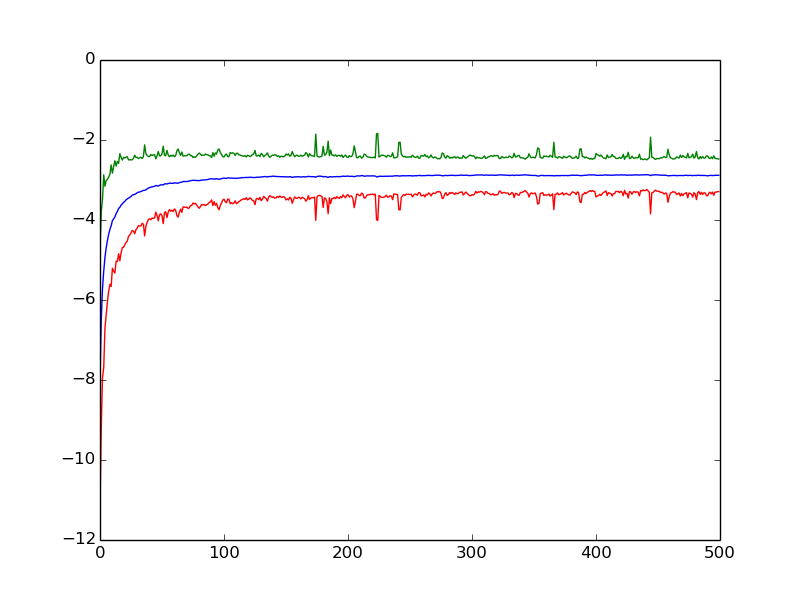
\includegraphics[width=\columnwidth]{../res/plot/helium_04/helium_04.png}
	\caption[caption]{$E_0$ vs. cycle number. 
	 	Trials: 4000. $\alpha = 1.79$. 
	$\beta = 0.4125$}
	\label{fig:helium_04}
\end{figure}
A problem that was encountred for all simulations was that the first samples of every 
trial were not valid samples for the ground state. This problem is not a problem for
Helium as the walkers quickly converges to a stage where they give correct
estimations of the ground state energy
as can be seen in figure (\ref{fig:helium_04}). 

\begin{figure}
	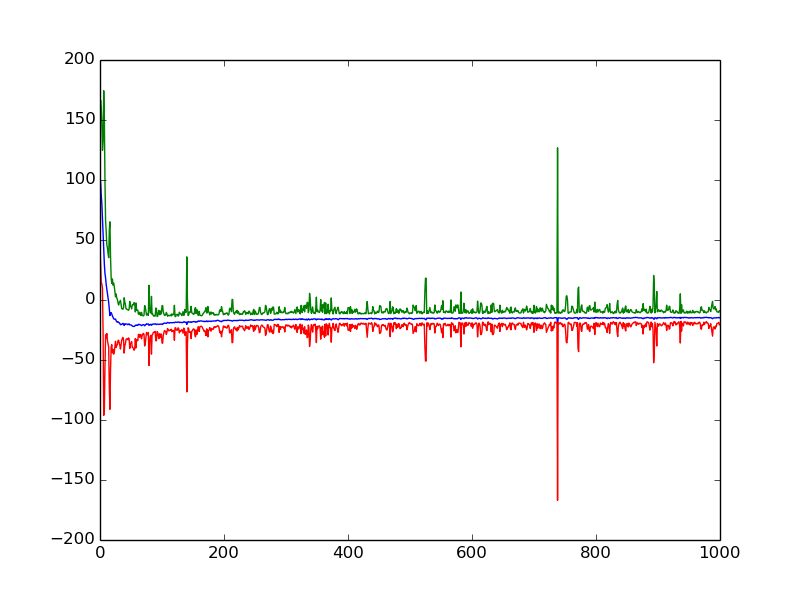
\includegraphics[width=\columnwidth]{../res/plot/beryllium_04/beryllium_04.png}
	\caption{Trials: 4000}
	\label{fig:beryllium_04}
\end{figure}
When increasing particle number and/or using GTOs this becomes an increasing problem
in addition with the increasing in CPU time used for every cycle. In the 
simulations of Beryllium and Neon the rate of which the samples begin to give
valid number for the ground state was increased to about 500 cycles. At 
Figure (\ref{fig:beryllium_04}) show the slow increase in the energy over cycle number. 

\subsection{Trial by Trial Variation}


\clearpage

\section{Results}
\subsection{Helium}
\subsubsection{Optimal Parameters}
\begin{figure}
	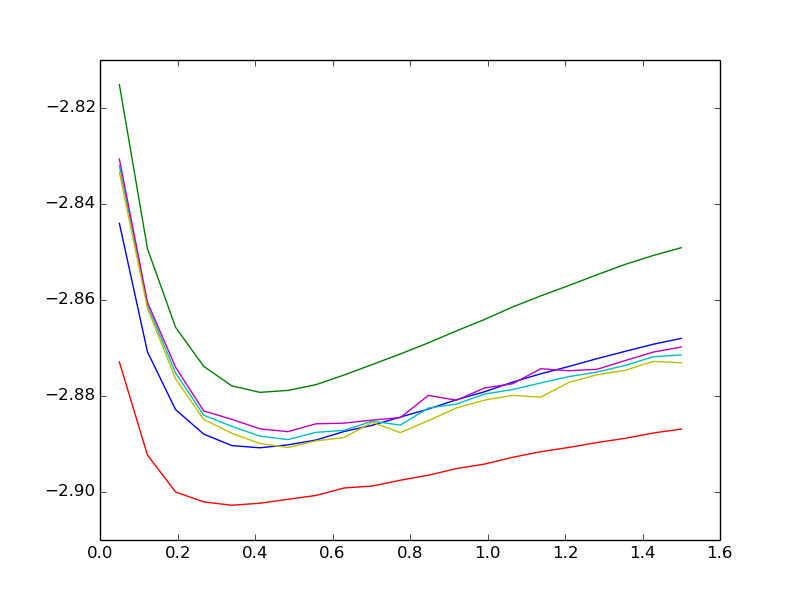
\includegraphics[width=\columnwidth]{../res/plot/helium_01/helium_01.png}
	\caption{Helium hydrogenlike wave function, 1 standard deviation. 
	Points = 20. Trials = 80.	$n_b = \:$1e5. $\alpha = 1.79$}
	\label{fig:helium_01}
\end{figure}
\begin{center}
	\begin{tabular}{| l a c a c |}
	\hline
		& Exact & $E_0$ & $\alpha$ & $\beta$\\
		w Imp. Sampl.& -2.90324 &  -2.89079& 1.79 & 0.4125 \\
		w/o Imp. Sampl. & -2.90324& -2.88864& 1.79 & 0.486 \\
		GTO 3-21G& -2.90324& & - & 0.9925\\
	\hline
	\end{tabular}
\end{center}
{\bf Importance Sampling:}

Importance sampling gave a lower estimation of the ground energy than
the simulation without it. Figure (\ref{fig:helium_01}) shows the difference between
running with and without importance sampling by varying the $\beta$ value. 
$\alpha$ is held constant at 1.79. 
The alpha was chosen to give the lowest energy of the simulation with 
importance sampling and the reason for doing this is that the evaluation of $E_0$ using
importance sampling is considered more correct.
The optimal values for Helium was found the be 
the similar for both importance sampling and with out, but not the same. 

From this point on all simulations will be done with importance sampling. \\

\noindent{\bf GTO Basis 3-21G :}

\begin{figure}
	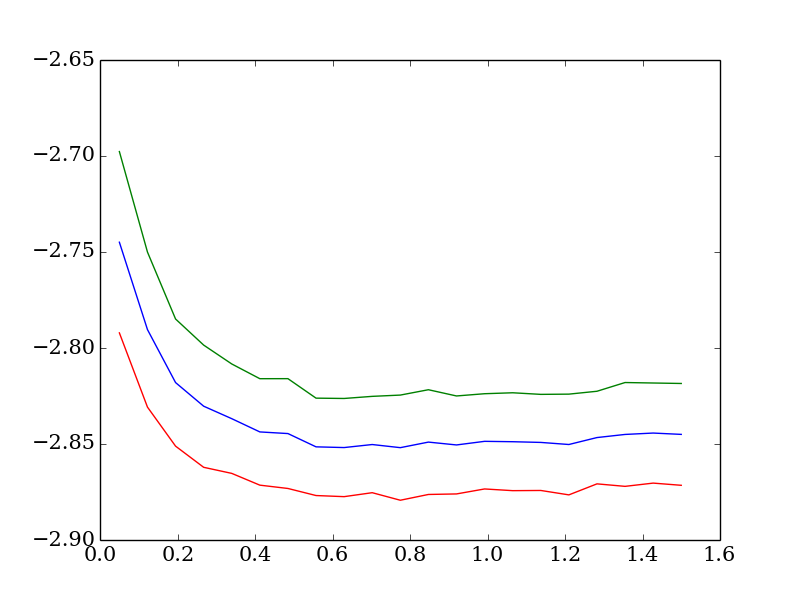
\includegraphics[width=\columnwidth]{../res/plot/helium_05/helium_05.png}
	\caption{Helium GTO importance sampling 1 standard deviation. 
	Points = 20. Trials = 40.	$n_b = \:$1e5.}
	\label{fig:helium_05}
\end{figure}
Figure (\ref{fig:helium_05}) shows the energy as a function of $\beta$. 
The lowest energy is $E_0 = 2.8519$. 
The variance is
roughly the same as with importance sampling
but $E_0$ has not decresead as one would expect. Because lower energies was
not discovered, even with more cycles, the implementation of the GTOs must be seen as flawed.

\subsubsection*{Charge Density}
\noindent{\bf Jastrow Factor:}

The Jastrow factor, which is a function of $\beta$, decides the interaction between
the electrons. Without this factor the electrons does not "see" the other electrons
in the system. This makes the electrons repulse each other and the charge density
is then push out from the nucleus as can be seen in figure(\ref{fig:helium_03}).
\begin{figure}
	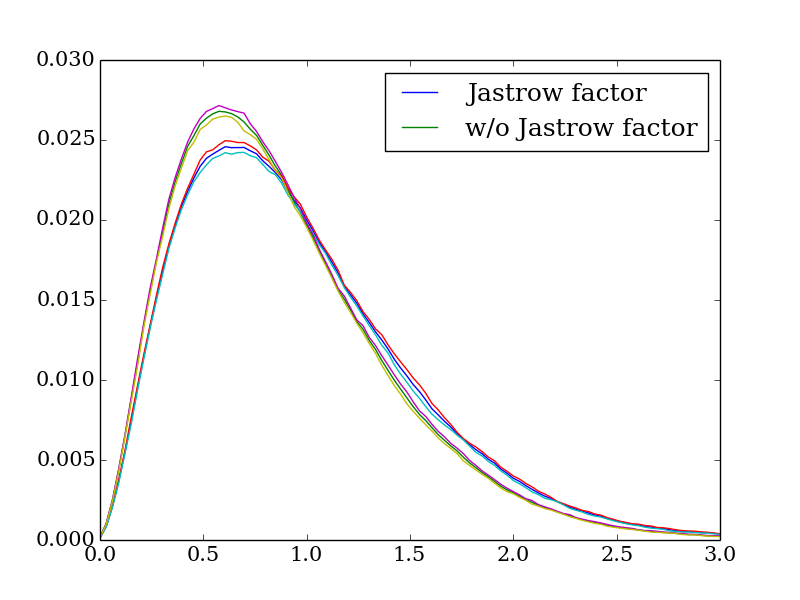
\includegraphics[width=\columnwidth]{../res/plot/helium_03/helium_03.png}
	\caption{Helium hydrogen like wave function, 1 standard deviation. 
	Points = 20. Trials = 40.	$n_b = \:$1e5.}
	\label{fig:helium_03}
\end{figure}

\subsection{Beryllium}
\subsubsection{Optimal Parameters}
\begin{center}
\begin{tabular}{| l a c a c |}
	\hline
		& Exact & $E_0$ & $\alpha$ & $\beta$\\
		Hydrogen like & -14.6664(3 &  -14.3795& 3.9190 & 0.01101 \\
		GTO 3-21G& -14.6664(3)& & - & 0.9925\\
	\hline
\end{tabular}	
\end{center}

\noindent 
The variance of the mean of $E_0$ makes it difficult to find optimal paramters.
The result is very dependent on how many cycles and how many trials are ryn.
For hydrogen like wave function the results were found to be:
\begin{align*}
	E_0 = -14.3795 && \alpha = 3.9190 && \beta = 0.110 && n_b = \text{1e5}&&\text{Trials} = 4 
\end{align*}

With adjusted paramters $E_0$ is lower using GTOs rather than hydrogen like 
wave functions. 



\begin{figure}
	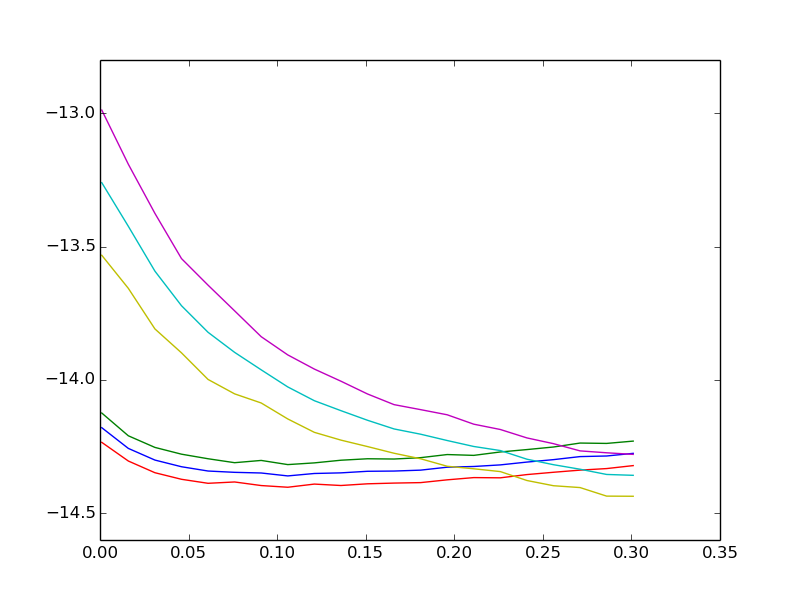
\includegraphics[width=\columnwidth]{../res/plot/beryllium_01/beryllium_01.png}
	\caption{Beryllium, 1 standard deviation. 
	Points = 20. Trials = 4.	$n_b = \:$1e5.}
	\label{fig:helium_03}
\end{figure}














\end{document}